\documentclass{article}
\usepackage{indentfirst}
\usepackage{graphicx}
\usepackage[utf8]{inputenc}
\usepackage{adjustbox}
\usepackage{float}
\usepackage{amsmath}
\usepackage{scrextend}
\usepackage{subfigure}

\usepackage{algorithm}
\usepackage[ruled,vlined]{algorithm2e}
\SetKwInput{KwInput}{Input}
\SetKwInput{KwOutput}{Output}

\usepackage{listings}
\usepackage{listings}
\lstset{
    language=Python,
    basicstyle=\ttfamily
}

\usepackage{longtable}
\usepackage{adjustbox}

\changefontsizes[15pt]{13pt}

\usepackage{hyperref}
\usepackage{geometry}
\geometry{legalpaper, margin=1.2in}

\usepackage[backend=biber]{biblatex}
\addbibresource{ref.bib}

\title{\LARGE \textbf{Analysis and Design of Algorithms: \\ 0/1 Knapsack Problem}}
\author{
    \begin{adjustbox}{width=.75\textwidth,center}
    \begin{tabular}{c c c}
      Ngo Bao Tran   &   \ Huynh Ngoc Tran  &  \ Nguyen Ngoc Khanh  \\
       18520173  & 18520385 &   18520901
    \end{tabular}
    \end{adjustbox}
}
\date{}

\begin{document}

\maketitle

\section{Introduction}
The Knapsack Problem is defined as: given an arrangement of objects, each with weight and a value, decide the number of each object to include in a capacity so that the total weight is little than a given capacity and the total value must as large as possible.

\subsection{Historical Background}
The knapsack problem seems to have first been identified in print in 1957, in two important publications. One was a paper by Geogre Dantzig (1957) \cite{dantzig}, one of the developers of linear programming and a creator of the field of Operations Research. He showed that the continuous version of the knapsack problem (the one faced by Bob) is perfectly maximized by choosing objects by bang-for-buck.

In the same year, Richard Bellman, another important early figure in Operations Research, described how to use dynamic programming to solve the knapsack problem. Very quickly thereafter the knapsack model was applied to a range of applications.

\subsection{Definition}
The 0-1 knapsack problem is defined as follows: Given a set of $n$ objects, each object $j$ having an integer value $v_j$ and an integer weight $w_j$. The problem is to choose a subset of the objects such that their overall value is maximized, while the overall weight does not exceed a given capacity $c$. We may formulate the model as the following integer programming model:\\
(KP) maximize $\sum\limits_{j = 1}^n v_j x_j$\\

\indent \indent subject to $\sum\limits_{j = 1}^n w_j x_j  \leq c$\\

\indent \indent \indent \indent \indent $x_j \in \{ 0, 1 \}, j = 1, ..., n$\\
where the binary decision variables $x_j$ are used to indicate whether object $j$ is included in the knapsack or not.
\subsection{Applications}
\indent Among the straightforward applications of the knapsack problem are, unsurprisingly, problems of loading shipping containers especially when one of weight or volume is known in advance to be the limiting constraint. These issues can be quite significant when space is scarce, as is the case when manufactured product is shipped to the US from China in advance of the holiday selling season.

Another common application is to cutting stock problems. For example, paper mills produce huge rolls of paper, the dimensions of which are determined by the manufacturing process. These roles are subsequently sliced into smaller rolls to fill customer orders. The value of the smaller rolls depends on the selling price. A similar problem is faced by manufacturers of fiber optic cable, who must decide how to cut lengths of cable to satisfy customer orders while extracting the greatest value from each length of cable.

In addition, the knapsack problem is a basic tool of portfolio optimization. The knapsack can be used to solve many scheduling problems. The knapsack also appears as a sub-problem in many, more complex mathematical models of real world problems. One general approach to difficult problems is to identify the most restrictive constraint, ignore the others, solve a knapsack problem, and somehow adjust the solution to satisfy ignored constraints. 
\subsection{An example of knapsack problem}
A merchant is packing his luggage on a trip to an auction. He wants to make as much profit as he can, since he loves money and wealth. He has some objects to sell, each has a weight and a value. Unfortunately, there are too many objects but his knapsack may not capable of carrying them all. So he must optimize his luggage - that is maximizing the total value while guaranteeing the overall weight not exceed the knapsack capacity. He hears that you are good at solving these kinds of problem. You shall help him with his luggage, maybe he will share the profit with you!

\textbf{INPUT}\\
The first input line contains two integers $\textbf{n}$ ($\mathbf{1 \leq n \leq 100}$) and $\mathbf{c}$ ($\mathbf{1 \leq c \leq 7000}$) - the number of objects and the knapsack capacity respectively.\\
The following $\textbf{n}$ lines each contains two integers $\textbf{w}$ and $\textbf{v}$ - the weight and the value of each object.

\textbf{OUTPUT}\\
A single integer denotes the greatest profit that can be achieved with the given capacity of the knapsack.
\section{Algorithms for Solving 0/1 Knapsack Problem}
\subsection{Observation}
\indent In order to solve this problem, we think about it as a sequence of choices. For each object we have two options: either to include it in the knapsack or not. To decide whether a choice is possible, we need to keep track of two pieces of information: \\
\indent 1. The remaining number of objects $i$ ($i \in [1, n]$)\\
\indent 2. The remaining capacity $c$ \\
\indent For the $i$-th object, we denote $w_i$ and $v_i$ as its weight and value respectively. We call such a pair $(i,c)$ a state of the problem. Each state corresponds to a subproblem that we denote by $V(i,c)$, with $V(i,c)$ is the maximum value we can obtain by selecting a subset of the objects (from the 1st to the $n$-th) from a knapsack of  capacity $C$. \\
\indent The original problem begins from the state $(n,C)$. At each state, we consider the choices we can make: \\
\indent 1. If the $i$-th object is not included, the optimal solution for the subproblem is $V(i-1, c)$. This is because we already made a decision for the $i$-th object and since we did not put it into the knapsack, we have the full capacity remaining for the other objects. \\
\indent 2. If the $i$-th object is included, the optimal solution for the subproblem is V(i-1, c-$w_i$). This is because we put the $i$-th object into the knapsack, so the knapsack capacity to put the remaining objects is reduced by the weight of the $i$-th object, $w_0$. \\
\indent We can generalize the problem by a recurrence relation between the subproblems:
\begin{equation}
    \centering
        V(i, c)= max\left\{
            \begin{array}{ll}
            V(i-1, c), & \mbox{if the $i$-th item is not included}.\\
            v_i + V(i-1, c-w_i), & \mbox{if the $i$-th item is included}.
            \end{array}
        \right.
\end{equation}
where $v_i$, $w_i$ denote the value and the weight of the $i$-th object respectively. \\
\indent At some point, the knapsack capacity may become negative, i.e., $c - w_i < 0$. Obviously, this means we can not include the $i$-th object in the knapsack since there is not enough capacity. Therefore, the optimal solution is $V(i-1, c)$. \\
\indent We also need initial conditions for the problem, which are: $V(0, c) = 0$ with $c \geq 0$ (no object to include in the knapsack) and $V(i, 0) = 0$ with $i \geq 0$ (no capacity available). 
From all those observations, we update the recurrence relation as follows:
\begin{equation}
   V(i, c)=
    \begin{cases}
      0, & \text{if $i = 0$ or $c = 0$}\\
      V(i-1, c), & \text{if $c-w_i < 0$}\\
      max(V(i-1, c), v_i + V(i-1, c-w_i)), & \text{otherwise}
    \end{cases}  
    \label{Eq.2}
\end{equation}

\subsection{Naive Recursive Solution}
\subsubsection{Approach}
A simple solution is to consider all subsets of items and calculate the total weight and value of all subsets, then consider only the subsets whose total weight is smaller than the capacity $C$. From all such subsets, pick the maximum value subset. \\
\indent With naive recursive solution, if there is a set of $n$ objects to choose from, then there will be $2^n$ possible combinations/subsets of objects (For each object, we have 2 choices: to include it it the subset or not. So, for the whole set of $n$ objects, there are a total of $2 \cdot 2 \cdot 2 \cdot ... \cdot 2$ ($n$ times) possible resulting subsets, all the way from the empty subset to the original set). 

\subsubsection{Pseudocode}
\begin{algorithm}[H]
\SetAlgoLined
\KwInput{\\
1. Number of items $n$ \\
2. Knapsack capacity $C$ \\
3. Array for $weights$, which holds the weights of all items \\
4. Array for $values$, which holds the values of all items}
\KwOutput{Maximum value that can be included in the knapsack}
Knapsack($n$, $C$, $weights$, $values$) \\
 \If{$n=0$ or $C=0$}{
   return 0\;
   }
 \eIf{$weights[n-1] > C$}{
   return Knapsack($n-1$, $C$, $weights$, $values$)\;
   }{
   return max($values[n-1]$ + Knapsack($n-1$, $C-weights[n-1]$, $weights$, $values$), Knapsack($n-1$, $C$, $weights$, $values$)\;
   }  
 \caption{Naive Recursive Solution}
\end{algorithm}

\subsubsection{Complexity Analysis}
\paragraph{Time Complexity}
We describe the runtime of this algorithm by the recurrence equation below
\begin{equation}
   T(n)=
    \begin{cases}
      c_1, & \text{if $n=0$}\\
      2T(n-1) + c_2, & \text{otherwise}
    \end{cases}       
    \label{Eq.3}
\end{equation}
\indent We solve this recurrence equation mathematically to analyse the runtime  complexity  of  the  algorithm. From (\ref{Eq.3}), we already have:
\begin{equation*}
    T(n) = 2T(n-1) + c_2
\end{equation*}
Thereby,
\begin{equation*}
    \begin{split}
        T(n) & = 2(2T(n-2) + c_2) + c_2 \\
        & = 2(2(2T(n-3) + c_2) + c_2) + c_2 \\
        & =2^r T(n-r) + c_2 \sum_{i=0}^{r-1} 2^i \\
        & = 2^r T(n-r) + (2^r - 1)c_2
    \end{split}
\end{equation*}
Putting $r = n$ gives
\begin{equation*}
    \begin{split}
        T(n) & = 2^n T(0) + (2^n - 1)c_2 \\
        & = 2^n (T(0) + c_2) - c_2 \\
        & = 2^n (c_1 + c_2) - c_2 \\
        & = O(2^n)
    \end{split}
\end{equation*}

\paragraph{Space Complexity} 
This algorithm uses $O(n)$ space to store the recursion call-stack. Since there is $n$ objects and our recursive algorith works in a depth-first fashion, which means, we can have maximum $n$ recursive calls on the call stack at any time. Therefore, the space complexity of the algorithm is $O(n)$.

\subsubsection{Source Code}
\begin{lstlisting}[breaklines=true]
def naive_recursion(num, capacity, w, v):
    #base conditions
     if num == 0 or capacity == 0: 
         return 0
    
     if w[num-1] > capacity:
         return f(num-1, capacity, w, v)

     else:
         return max(v[num-1] + f(num-1, capacity-w[num-1],w ,v), f(num-1, capacity, w, v))
\end{lstlisting}

\subsection{Top-down Dynamic Programming}
\subsubsection{Approach}
Though naive recursive solution is a simple approach, it runs very slow. This is because the algorithm considers 2 options for every object in the original set, which means at each state $(i, c)$, it makes 2 recursive calls. Thus, the total number of recursive calls is $O(2^n)$. \\
\indent In fact, the total number of state $(i,c)$ that need to be considered is $n \cdot C$. Since there are $O(2^n)$ recursive calls and each of them corresponds to a state, if $2^n > n \cdot C$ (which is always true with $n \geq 0$ and $C \geq 0$), there must be some repeated recursive calls. In other words, some states are uselessly computed several times. \\
\indent To avoid this repetition, we adopt memoization technique \cite{memo}. We store the result of each recursive call in a table. At each state $(i,c)$, we store its calculated result if we get it the first time. Afterwards, if we come across the same state $(i,c)$ again, instead of calculating it in exponential complexity we can directly return its result stored in the table in constant time. \\
\indent The value of each state is computed using the similar recurrence relation as (\ref{Eq.2}).

\subsubsection{Pseudocode}
\begin{algorithm}[H]
\SetAlgoLined
\KwInput{\\
1. Number of items $n$ \\
2. Knapsack capacity $C$ \\
3. Array for $weights$, which holds the weights of all items \\
4. Array for $values$, which holds the values of all items}
\KwOutput{Maximum value that can be included in the knapsack}
dpKnapsack($n$, $C$, $weights$, $values$) \\
initialize $memoi[][]$ of size $(n+1)\cdot (C+1)$ \; \\
 \If{$n=0$ or $C=0$}{
   return 0\;
   }
  \If{$memoi[n][C] \neq 0$}{
    return $memoi[n][C]$\;
  }
 \eIf{$weights[n-1] > C$}{
   $memoi[n][C]$ = dpKnapsack($n-1$, $C$, $weights$, $values$)\;
   return $memoi[n][C]$\;
   }{
   $memoi[n][C]$ =  max($values[n-1]$ + dpKnapsack($n-1$, $C-weights[n-1]$, $weights$, $values$), dpKnapsack($n-1$, $C$, $weights$, $values$)\;
   return $memoi[n][C]$\;
   }  
 \caption{Top-down Dynamic Programming}
\end{algorithm}

\subsubsection{Complexity Analysis}
\paragraph{Time Complexity}
In this method, since there are $n \cdot C$ states, each state is only computed once and each call takes constant time $c$, the time complexity can be generalized with the formula: 
\begin{equation}
    \begin{split}
        \sum_{i=1}^{n} \sum_{j=1}^{C} c & = \sum_{i=1}^{n} (c + c + ... + c) \; \text{($C$ times)} \\
        & = C \cdot c \cdot (c + c + ... + c) \; \text{($n$ times)} \\
        & = n \cdot C \cdot c^2 \\
        & = O(n \cdot C)
    \end{split}
    \label{Eq.4}
\end{equation}

\paragraph{Space Complexity}
Since the memoization array is of size $(n+1) \cdot (C+1)$, the algorithm uses $O(n\cdot C)$ space for this. (This can be proved similarly to Equation (\ref{Eq.5})). In addition, there is $O(n)$ space used for the recursion call-stack. Therefore, the total space complexity of the algorithm is $O(n\cdot C + n)$, which is asymptotically equivalent to $O(n\cdot C)$.

\subsubsection{Source Code}
\begin{lstlisting}[breaklines=true]
def topdown_dpKnapsack(num, capacity, w, v): 
    #initialization
    memoi = [[0 for x in range(capacity + 1)] for x in range(num + 1)]
    
    #base conditions
    if num == 0 or capacity == 0:   
        return 0
    if memoi[num][capacity] != 0:
        return memoi[num][capacity]
    
    if w[num-1] > capacity:
        #store the value of function call before return 
        memoi[num][capacity] = f(num-1, capacity, w, v)
        return memoi[num][capacity]
    else:
        #store the value of function call before return
        memoi[num][capacity] = max(v[num-1] + f(num-1, capacity-w[num-1], w, v), f(num-1, capacity, w, v))
        return memoi[num][capacity]
\end{lstlisting}

\subsection{Bottom-up Dynamic Programming}
\subsubsection{Approach}
In the previous section, we have discussed about top-down dynamic programming, which is a combination of recursion and memoization. There is another way to implement dynamic programming to solve 0/1 knapsack problem. \\
\indent In the top-down solution, we defined the states and subproblems starting from the original problem that we want to solve, which is having all objects available and a knapsack of capacity $C$. However, in bottom-up approach, we start from the smallest subproblems and iteratively increase the size and compute the new solutions from the ones we already know. We construct a temporary table of size $(n+1)\cdot(C+1)$ to store the values of all states, from $(0,0)$ to $(n,C)$. The value at each state is denoted as $V(i,c)$ and is computed by the similar recurrence relation (\ref{Eq.2}).

\subsubsection{Pseudocode}
\begin{algorithm}[H]
\SetAlgoLined
\KwInput{\\
1. Number of items $n$ \\
2. Knapsack capacity $C$ \\
3. Array for $weights$, which holds the weights of all items \\
4. Array for $values$, which holds the values of all items}
\KwOutput{Maximum value that can be included in the knapsack}
dpKnapsack($n$, $C$, $weights$, $values$) \\
initialize $memoi[][]$ of size $(n+1)\cdot (C+1)$\; \\
\For{$i \in [0, n]$}{
    \For{$j \in [0, C]$}{
        \If{$i = 0$ or $j = 0$}{
            $memoi[i][j] = 0$\;}
        \eIf{$weights[i-1] \leq j$}{
            $memoi[i][j]$ =  max($values[i-1]$ + $memoi[i-1][j-weights[i-1]]$, $memoi[i-1][j]$\;}{
        $memoi[i][j] = memoi[i-1][j]$\;}
        $j++$ \; \\
        }
    $i++$ \; \\
    }
return $memoi[n][C]$ \;
 \caption{Bottom-up Dynamic Programming}
\end{algorithm}

\subsubsection{Complexity Analysis}
\paragraph{Time Complexity}
The bottom-up algorithm fills a table of size $(n+1)\cdot(C+1)$, filling each cell of the table takes constant time using equation (\ref{Eq.2}). Therefore, the runtime complexity can be generalized as the formula
\begin{equation}
    \begin{split}
      \sum_{i=0}^{n} \sum_{j=0}^{C} c & = \sum_{i=1}^{n} (c + c + ... + c) \; \text{($C+1$ times)} \\
        & = (C+1) \cdot c \cdot (c + c + ... + c) \; \text{($n+1$ times)} \\
        & = (n+1) \cdot (C+1) \cdot c^2 \\
        & = O(n \cdot C)  
    \end{split}
    \label{Eq.5}
\end{equation}

\paragraph{Space Complexity}
Since the memoization array is of size $(n+1) \cdot (C+1)$, the algorithm space complexity is $O(n\cdot C)$. (This can be proved similarly to Equation (\ref{Eq.5})).

\subsubsection{Source Code}
\begin{lstlisting}[breaklines=true]
def bottomup_dpKnapsack(num, capacity, w, v, memoi):
    #initialization
    memoi = [[0 for x in range(capacity + 1)] for x in range(num + 1)]
    
    #build table in bottom-up manner
    for i in range(num + 1): 
        for j in range(capacity + 1): 
            if i == 0 or j == 0: 
                memoi[i][j] = 0
            elif w[i-1] <= j:
                memoi[i][j] = max(v[i-1] + memoi[i-1][j-w[i-1]], memoi[i-1][j]) 
            else: 
                memoi[i][j] = memoi[i-1][j]
    return memoi[num][capacity]
\end{lstlisting}

\section{Test cases to check correctness of algorithm}
In order to guarantee the correctness of those algorithms that we implemented, we used some test cases to compare the output results. Test cases can be divided into three main categories:
\begin{itemize}
    \item \textbf{Base Cases}: there are two remarkable cases as below.
    \begin{itemize}
        \item When the knapsack is not capable of carrying any object, which means $w_j > C$ for $j = 1, ..., n$.\\
        Example:\\
        5 10\\
        20 30\\
        12 15\\
        15 8\\
        30 3\\
        18 25
        \item When the knapsack is capable of carrying all objects, which means $\sum\limits_{j = 1}^n w_j \leq C$.\\
        Example:\\
        5 100\\
        20 30\\
        12 15\\
        15 8\\
        30 3\\
        18 25
    \end{itemize}
    \item \textbf{Edge Cases}: when $n = 100$ and $C = 7000$.
    \item \textbf{Normal Cases}: when $0 < n < 100$ and $ 0 < C < 7000$. All weights are smaller than the capacity $C$, and the overall weight of the objects exceeds $C$.\\
    Example:\\
    \textbf{Input}\\
    6 190\\
    56 50\\
    59 50\\
    80 64\\
    64 46\\
    75 50\\
    17 5\\
    \textbf{Output} (the first, second and fifth object are chosen)\\
    Top-down dynamic programming:\\
    150 \\
    1 1 0 0 1 0  \\
    Bottom-up dynamic programming:\\
    150 \\
    1 1 0 0 1 0
\end{itemize}

For the normal cases, we use a dataset called KNAPSACK\_01, which is available on \cite{knapsack01} and refers to \cite{vance93}. This is a dataset directory which contains some examples of data for 0-1 knapsack problems. It contains 8 tests in which $n$ varies from 5 to 24 and $c$ from 26 to 6404180. Each test has four files which contain the knapsack capacity, the weights of the objects, the values of each object and the optimal selection of weights.\\

For example, \textbf{P01} is a set of 10 weights and values for a knapsack of capacity 165.
\begin{itemize}
    \item p01\_c.txt, the knapsack capacity, which is 165.
    \item p01\_w.txt, the weights of the objects. The file contains a list of \{23, 31, 29, 44, 53, 38, 63, 85, 89, 82\}.
    \item p01\_p.txt, the value of each object. The file contains a list of \{92, 57, 49, 68, 60, 43, 67, 84, 87, 72\}.
    \item p01\_s.txt, the optimal selection of weights. The file contains a list of \{1, 1, 1, 1, 0, 1, 0, 0, 0, 0\}, where '1' indicates the object is chosen and vice versa.
\end{itemize}

\section{Experiments}
We compute the real runtime of top-down and bottom-up dynamic programming by profiling the scripts. To evaluate the time complexity of the algorithm, we consider its running time to be defined as $T(n,C) = af(n,C) + b$, where $f(n,C)$ is a runtime complexity function. Then, we compute the values of $a$ and $b$ for each case of $f(n,C)$ by applying Linear Regression algorithm, with Mean Square Error (MSE) as the residual standard deviation. The results are shown in the tables below.\\

\indent $\bullet$ \textbf{Top-down dynamic programming}
\begin{center}
\begin{table}[H]
    \begin{adjustbox}{width=1.1\textwidth,center}
        \begin{tabular}{|c|c|c|c|c|c|c|c|}
        \hline
        {} & $log_2(x)$ & $sqrt(x)$ & $x$ & $xlog_2(x)$ & $x^2$ & $x^3$ & $2^x$ \\
        \hline
        a & 62.15103	&	0.73303	&	8.26970E-04	&	4.24393E-05	&	1.14153E-09	&	1.95031E-15	&	1	\\ 	\hline
        b & -841.04006	&	-119.31452	&	-8.39906	&	1.46416	&   6.94126E+01	&	6.72927E-32	&	 0	\\ 	\hline
        \end{tabular}
    \end{adjustbox}
    \caption{Values of $a$ and $b$ for each case of $f(n,C)$ ($x = n\cdot C)$}.
\end{table}
    \setlength{\LTleft}{-20cm plus -1.5fill}
    \setlength{\LTright}{\LTleft}
    \begin{longtable}{|c|c|c|c|c|c|c|c|c|c|c|}
    \hline
        $n$ & $C$ & runtime & memory & $log_2(x)$ & $sqrt(x)$ & $x$ & $xlog_2(x)$ & $x^2$ & $x^3$ & $2^x$ \\
        \hline
3	&	200	&	0.039	&	1354.077	&	-267.459	&	-101.359	&	-7.903	&	1.699	&	69.413	&	4.21E-07	&	4.15E+180	\\	\hline
5	&	300	&	0.136	&	16.894	&	-185.300	&	-90.925	&	-7.159	&	2.136	&	69.415	&	6.58E-06	&	3.51E+451	\\	\hline
6	&	350	&	0.242	&	1509.128	&	-155.130	&	-85.723	&	-6.662	&	2.448	&	69.418	&	1.81E-05	&	1.46E+632	\\	\hline
9	&	500	&	0.902	&	1536.275	&	-86.793	&	-70.142	&	-4.678	&	3.782	&	69.436	&	1.78E-04	&	4.32E+1354	\\	\hline
10	&	550	&	1.301	&	227.369	&	-68.800	&	-64.952	&	-3.851	&	4.364	&	69.447	&	3.24E-04	&	4.62E+1655	\\	\hline
12	&	650	&	2.183	&	1573.934	&	-37.473	&	-54.575	&	-1.949	&	5.744	&	69.482	&	9.26E-04	&	1.08E+2348	\\	\hline
15	&	800	&	4.652	&	1657.908	&	1.153	&	-39.015	&	1.525	&	8.365	&	69.577	&	3.37E-03	&	2.29E+3612	\\	\hline
18	&	950	&	7.355	&	1732.370	&	32.910	&	-23.459	&	5.742	&	11.669	&	69.746	&	9.75E-03	&	4.10E+5147	\\	\hline
20	&	1050	&	9.683	&	505.720	&	51.331	&	-13.089	&	8.967	&	14.260	&	69.916	&	1.81E-02	&	4.26E+6321	\\	\hline
21	&	1100	&	11.653	&	1828.476	&	59.877	&	-7.904	&	10.704	&	15.675	&	70.022	&	2.40E-02	&	6.21E+6953	\\	\hline
24	&	1250	&	16.119	&	1962.313	&	83.312	&	7.649	&	16.410	&	20.400	&	70.440	&	5.27E-02	&	7.94E+9030	\\	\hline
25	&	1300	&	17.427	&	750.145	&	90.489	&	12.834	&	18.477	&	22.137	&	70.618	&	6.70E-02	&	2.98E+9783	\\	\hline
27	&	1400	&	23.199	&	2138.013	&	104.035	&	23.202	&	22.860	&	25.858	&	71.044	&	1.05E-01	&	8.59E+11378	\\	\hline
30	&	1550	&	27.908	&	2260.110	&	122.608	&	38.754	&	30.055	&	32.062	&	71.881	&	1.96E-01	&	7.85E+13997	\\	\hline
33	&	1700	&	37.931	&	2522.056	&	139.437	&	54.306	&	37.994	&	39.024	&	73.005	&	3.44E-01	&	6.06E+16887	\\	\hline
35	&	1800	&	40.086	&	1343.501	&	149.838	&	64.674	&	43.700	&	44.091	&	73.943	&	4.88E-01	&	7.76E+18964	\\	\hline
36	&	1850	&	44.750	&	2665.195	&	154.821	&	69.858	&	46.677	&	46.753	&	74.476	&	5.76E-01	&	3.96E+20048	\\	\hline
39	&	2000	&	55.207	&	2910.428	&	168.988	&	85.409	&	56.105	&	55.260	&	76.358	&	9.26E-01	&	2.19E+23480	\\	\hline
40	&	2050	&	51.208	&	1620.455	&	173.472	&	90.592	&	59.412	&	58.270	&	77.088	&	1.08E+00	&	2.88E+24684	\\	\hline
42	&	2150	&	66.374	&	3227.356	&	182.118	&	100.960	&	66.276	&	64.553	&	78.721	&	1.44E+00	&	1.02E+27183	\\	\hline
45	&	2300	&	75.528	&	3309.013	&	194.351	&	116.511	&	77.192	&	74.639	&	81.641	&	2.16E+00	&	4.02E+31156	\\	\hline
48	&	2450	&	89.651	&	3760.036	&	205.803	&	132.061	&	88.853	&	85.528	&	85.200	&	3.17E+00	&	1.34E+35401	\\	\hline
50	&	2550	&	87.576	&	2659.872	&	213.050	&	142.428	&	97.040	&	93.236	&	87.970	&	4.04E+00	&	2.11E+38381	\\	\hline
51	&	2600	&	95.487	&	3867.320	&	216.567	&	147.612	&	101.257	&	97.225	&	89.484	&	4.55E+00	&	3.77E+39916	\\	\hline
54	&	2750	&	120.072	&	4439.771	&	226.721	&	163.163	&	114.406	&	109.737	&	94.586	&	6.39E+00	&	9.00E+44702	\\	\hline
55	&	2800	&	103.664	&	3154.096	&	229.982	&	168.346	&	118.954	&	114.090	&	96.485	&	7.12E+00	&	4.16E+46358	\\	\hline
57	&	2900	&	132.511	&	4681.433	&	236.331	&	178.713	&	128.299	&	123.071	&	100.604	&	8.81E+00	&	1.81E+49760	\\	\hline
60	&	3050	&	136.911	&	4959.332	&	245.452	&	194.263	&	142.936	&	137.232	&	107.641	&	1.20E+01	&	3.09E+55088	\\	\hline
63	&	3200	&	158.034	&	5432.929	&	254.132	&	209.814	&	158.318	&	152.226	&	115.807	&	1.60E+01	&	4.44E+60687	\\	\hline
65	&	3300	&	152.067	&	4367.104	&	259.693	&	220.181	&	168.986	&	162.688	&	121.935	&	1.92E+01	&	8.59E+64570	\\	\hline
66	&	3350	&	176.070	&	5874.163	&	262.411	&	225.364	&	174.444	&	168.059	&	125.216	&	2.11E+01	&	5.40E+66557	\\	\hline
69	&	3500	&	197.876	&	6347.402	&	270.324	&	240.914	&	191.314	&	184.735	&	135.989	&	2.75E+01	&	5.55E+72698	\\	\hline
70	&	3550	&	178.678	&	5167.893	&	272.886	&	246.098	&	197.103	&	190.482	&	139.904	&	2.99E+01	&	8.99E+74805	\\	\hline
72	&	3650	&	199.231	&	6428.397	&	277.903	&	256.465	&	208.929	&	202.259	&	148.251	&	3.54E+01	&	4.82E+79110	\\	\hline
75	&	3800	&	222.596	&	7120.902	&	285.174	&	272.015	&	227.287	&	220.637	&	162.133	&	4.51E+01	&	3.54E+85793	\\	\hline
78	&	3950	&	273.514	&	7930.211	&	292.162	&	287.565	&	246.390	&	239.871	&	177.773	&	5.70E+01	&	2.19E+92747	\\	\hline
80	&	4050	&	246.679	&	6655.201	&	296.674	&	297.932	&	259.539	&	253.173	&	189.245	&	6.63E+01	&	5.23E+97533	\\	\hline
81	&	4100	&	276.148	&	8020.428	&	298.888	&	303.115	&	266.238	&	259.968	&	195.312	&	7.14E+01	&	1.15E+99972	\\	\hline
84	&	4250	&	302.934	&	8829.177	&	305.371	&	318.665	&	286.829	&	280.930	&	214.899	&	8.87E+01	&	5.11E+107467	\\	\hline
85	&	4300	&	264.954	&	7432.936	&	307.481	&	323.849	&	293.859	&	288.110	&	221.909	&	9.52E+01	&	2.91E+110026	\\	\hline
87	&	4400	&	308.473	&	8924.333	&	311.627	&	334.215	&	308.165	&	302.762	&	236.687	&	1.09E+02	&	1.92E+115234	\\	\hline
90	&	4550	&	351.806	&	9681.838	&	317.673	&	349.766	&	330.245	&	325.468	&	260.835	&	1.34E+02	&	6.07E+123271	\\	\hline
93	&	4700	&	371.533	&	10141.364	&	323.521	&	365.316	&	353.070	&	349.051	&	287.509	&	1.63E+02	&	1.63E+131580	\\	\hline
95	&	4800	&	348.182	&	9528.903	&	327.317	&	375.682	&	368.699	&	365.262	&	306.777	&	1.85E+02	&	4.77E+137269	\\	\hline
96	&	4850	&	386.927	&	10974.432	&	329.185	&	380.866	&	376.638	&	373.515	&	316.876	&	1.97E+02	&	3.68E+140159	\\	\hline
99	&	5000	&	398.530	&	11177.588	&	334.675	&	396.416	&	400.951	&	398.864	&	349.115	&	2.37E+02	&	7.05E+149009	\\	\hline
100	&	5050	&	380.614	&	10170.228	&	336.469	&	401.599	&	409.221	&	407.510	&	360.530	&	2.51E+02	&	1.41E+152020	\\	\hline
102	&	5150	&	440.264	&	11998.021	&	340.003	&	411.966	&	426.008	&	425.100	&	384.405	&	2.83E+02	&	1.14E+158131	\\	\hline
105	&	5300	&	481.533	&	12734.855	&	345.176	&	427.516	&	451.810	&	452.228	&	422.934	&	3.36E+02	&	1.56E+167523	\\	\hline
108	&	5450	&	485.159	&	13387.324	&	350.204	&	443.066	&	478.356	&	480.250	&	464.894	&	3.98E+02	&	1.80E+177186	\\	\hline
110	&	5550	&	484.742	&	12820.410	&	353.480	&	453.432	&	496.466	&	499.429	&	494.871	&	4.44E+02	&	6.49E+183778	\\	\hline
111	&	5600	&	508.598	&	13721.426	&	355.096	&	458.616	&	505.646	&	509.169	&	510.483	&	4.68E+02	&	1.76E+187120	\\	\hline
114	&	5750	&	564.509	&	14770.801	&	359.857	&	474.166	&	533.680	&	538.989	&	559.904	&	5.49E+02	&	1.45E+197325	\\	\hline
115	&	5800	&	470.064	&	12663.352	&	361.416	&	479.349	&	543.190	&	549.129	&	577.265	&	5.79E+02	&	1.01E+200787	\\	\hline
117	&	5900	&	598.635	&	15561.301	&	364.495	&	489.716	&	562.458	&	569.712	&	613.366	&	6.42E+02	&	1.01E+207801	\\	\hline
120	&	6050	&	613.842	&	16294.172	&	369.016	&	505.266	&	591.981	&	601.341	&	671.084	&	7.46E+02	&	5.98E+218547	\\	\hline
125	&	6300	&	618.357	&	16351.694	&	376.307	&	531.182	&	642.840	&	656.078	&	777.337	&	9.52E+02	&	1.32E+237061	\\	\hline

     \caption{The real runtime of the algorithm and the values of $T(n,C)$ computed by $af(n,C) + b$ with different values of $n$ and $C$ ($x = n\cdot C)$}
    \end{longtable}
\begin{table}[H]
    \begin{adjustbox}{width=1.1\textwidth,center}
         \begin{tabular}{|c|c|c|c|c|c|c|c|}
        \hline
        {} & $log_2(x)$ & $sqrt(x)$ & $x$ & $xlog_2(x)$ & $x^2$ & $x^3$ & $2^x$ \\
        \hline
        MSE & 13046.395	&	2595.901	&	277.039	&	292.535	&	3217.342	&	15800	&	3.89E+474120  \\  \hline
        \end{tabular}
    \end{adjustbox}
    \caption{MSE for each case of $f(n,C)$ ($x = n\cdot C)$} 
\end{table}    
\end{center}

\indent $\bullet$ \textbf{Bottom-up dynamic programming}

\begin{center}
\begin{table}[H]
    \begin{adjustbox}{width=1.1\textwidth,center}
        \begin{tabular}{|c|c|c|c|c|c|c|c|}
        \hline
        {} & $log_2(x)$ & $sqrt(x)$ & $x$ & $xlog_2(x)$ & $x^2$ & $x^3$ & $2^x$ \\
        \hline
        a & 58.561395	&	0.83347	&	1.15254E-03	&	6.09185E-05	&	2.29557E-09	&	5.05673E-15	&	0	\\ 	\hline
        b & -762.35905	&	-108.41879	&	-4.40603	&	5.26812	&	7.14839E+01	&	6.72927E-32	&	 187.20966	\\ 	\hline
        \end{tabular}
    \end{adjustbox}
    \caption{Values of $a$ and $b$ for each case of $f(n,C)$ ($x = n\cdot C)$}.
\end{table}
    \setlength{\LTleft}{-25cm plus -1fill}
    \setlength{\LTright}{\LTleft}
    \begin{longtable}{|c|c|c|c|c|c|c|c|c|c|c|}
    \hline
        $n$ & $C$ & runtime & memory & $log_2(x)$ & $sqrt(x)$ & $x$ & $xlog_2(x)$ & $x^2$ & $x^3$ & $2^x$ \\
        \hline
3	&	200	&	0.346	&	12515.918	&	-221.907	&	-88.003	&	-3.715	&	5.605	&	8.26E+05	&	9.17E-04	&	187.210	\\	\hline
 5	&	300	&	1.014	&	1271.969	&	-144.493	&	-76.139	&	-2.677	&	6.232	&	5.17E+06	&	1.86E-05	&	187.210	\\	\hline
6	&	350	&	1.621	&	12643.732	&	-116.065	&	-70.224	&	-1.986	&	6.680	&	1.01E+07	&	9.52E-03	&	187.210	\\	\hline
9	&	500	&	4.032	&	12644.857	&	-51.675	&	-52.508	&	0.780	&	8.595	&	4.65E+07	&	5.10E-02	&	187.210	\\	\hline
10	&	550	&	5.008	&	1399.937	&	-34.721	&	-46.607	&	1.933	&	9.431	&	6.94E+07	&	1.89E-01	&	187.210	\\	\hline
12	&	650	&	7.246	&	12645.422	&	-5.204	&	-34.809	&	4.584	&	11.412	&	1.40E+08	&	5.54E-01	&	187.210	\\	\hline
15	&	800	&	11.674	&	1399.358	&	31.192	&	-17.117	&	9.424	&	15.174	&	3.31E+08	&	1.38E+00	&	187.210	\\	\hline
18	&	950	&	17.065	&	12646.008	&	61.114	&	0.571	&	15.302	&	19.916	&	6.71E+08	&	3.04E+00	&	187.210	\\	\hline
20	&	1050	&	21.472	&	1399.311	&	78.471	&	12.362	&	19.797	&	23.636	&	1.01E+09	&	6.11E+00	&	187.210	\\	\hline
21	&	1100	&	23.678	&	12645.889	&	86.524	&	18.257	&	22.218	&	25.667	&	1.22E+09	&	1.14E+01	&	187.210	\\	\hline
24	&	1250	&	30.942	&	12646.519	&	108.606	&	35.942	&	30.170	&	32.449	&	2.07E+09	&	2.01E+01	&	187.210	\\	\hline
25	&	1300	&	33.915	&	1399.725	&	115.368	&	41.837	&	33.051	&	34.942	&	2.42E+09	&	3.38E+01	&	187.210	\\	\hline
27	&	1400	&	39.476	&	12647.047	&	128.131	&	53.626	&	39.160	&	40.284	&	3.28E+09	&	5.44E+01	&	187.210	\\	\hline
30	&	1550	&	49.778	&	1400.216	&	145.632	&	71.309	&	49.187	&	49.189	&	4.96E+09	&	8.45E+01	&	187.210	\\	\hline
33	&	1700	&	59.270	&	12647.619	&	161.489	&	88.992	&	60.251	&	59.182	&	7.22E+09	&	1.28E+02	&	187.210	\\	\hline
35	&	1800	&	68.025	&	1399.974	&	171.289	&	100.780	&	68.204	&	66.455	&	9.11E+09	&	1.87E+02	&	187.210	\\	\hline
36	&	1850	&	70.642	&	12648.143	&	175.984	&	106.674	&	72.353	&	70.277	&	1.02E+10	&	2.69E+02	&	187.210	\\	\hline
39	&	2000	&	83.936	&	12648.322	&	189.333	&	124.356	&	85.492	&	82.488	&	1.40E+10	&	3.78E+02	&	187.210	\\	\hline
40	&	2050	&	90.259	&	1400.696	&	193.558	&	130.250	&	90.102	&	86.808	&	1.54E+10	&	5.22E+02	&	187.210	\\	\hline
42	&	2150	&	96.684	&	12647.928	&	201.704	&	142.038	&	99.668	&	95.827	&	1.87E+10	&	7.09E+02	&	187.210	\\	\hline
45	&	2300	&	114.811	&	1401.084	&	213.231	&	159.720	&	114.882	&	110.306	&	2.46E+10	&	9.49E+02	&	187.210	\\	\hline
48	&	2450	&	128.511	&	12501.223	&	224.021	&	177.401	&	131.132	&	125.935	&	3.17E+10	&	1.86E-05	&	187.210	\\	\hline
50	&	2550	&	142.531	&	1402.377	&	230.850	&	189.189	&	142.542	&	136.999	&	3.73E+10	&	9.17E-04	&	187.210	\\	\hline
51	&	2600	&	144.401	&	12501.418	&	234.164	&	195.083	&	148.420	&	142.726	&	4.04E+10	&	9.52E-03	&	187.210	\\	\hline
54	&	2750	&	162.607	&	12501.762	&	243.732	&	212.764	&	166.746	&	160.686	&	5.06E+10	&	5.10E-02	&	187.210	\\	\hline
55	&	2800	&	171.898	&	1401.970	&	246.804	&	218.658	&	173.085	&	166.935	&	5.44E+10	&	1.89E-01	&	187.210	\\	\hline
57	&	2900	&	182.248	&	12501.376	&	252.787	&	230.445	&	186.108	&	179.826	&	6.27E+10	&	5.54E-01	&	187.210	\\	\hline
60	&	3050	&	205.512	&	1403.288	&	261.381	&	248.126	&	206.508	&	200.153	&	7.69E+10	&	1.38E+00	&	187.210	\\	\hline
63	&	3200	&	223.508	&	12502.288	&	269.559	&	265.808	&	227.945	&	221.676	&	9.33E+10	&	3.04E+00	&	187.210	\\	\hline
65	&	3300	&	243.473	&	1403.758	&	274.799	&	277.595	&	242.813	&	236.693	&	1.06E+11	&	1.19E-06	&	187.210	\\	\hline
66	&	3350	&	246.929	&	12503.438	&	277.360	&	283.489	&	250.420	&	244.403	&	1.12E+11	&	5.10E-05	&	187.210	\\	\hline
69	&	3500	&	269.829	&	12502.854	&	284.816	&	301.170	&	273.932	&	268.340	&	1.34E+11	&	5.02E-04	&	187.210	\\	\hline
70	&	3550	&	282.545	&	1403.459	&	287.230	&	307.063	&	281.999	&	276.589	&	1.42E+11	&	2.61E-03	&	187.210	\\	\hline
72	&	3650	&	293.525	&	12503.675	&	291.957	&	318.851	&	298.481	&	293.495	&	1.59E+11	&	2.75E-02	&	187.210	\\	\hline
75	&	3800	&	324.591	&	1404.024	&	298.809	&	336.532	&	324.067	&	319.874	&	1.86E+11	&	6.79E-02	&	187.210	\\	\hline
78	&	3950	&	346.326	&	12504.205	&	305.393	&	354.212	&	350.691	&	347.484	&	2.18E+11	&	1.49E-01	&	187.210	\\	\hline
80	&	4050	&	373.451	&	1404.125	&	309.644	&	366.000	&	369.016	&	366.577	&	2.41E+11	&	2.98E-01	&	187.210	\\	\hline
81	&	4100	&	373.443	&	12503.741	&	311.731	&	371.893	&	378.352	&	376.331	&	2.53E+11	&	9.73E-01	&	187.210	\\	\hline
84	&	4250	&	400.707	&	12504.520	&	317.839	&	389.574	&	407.050	&	406.421	&	2.93E+11	&	1.63E+00	&	187.210	\\	\hline
85	&	4300	&	421.900	&	1404.912	&	319.827	&	395.468	&	416.846	&	416.728	&	3.07E+11	&	2.61E+00	&	187.210	\\	\hline
87	&	4400	&	429.813	&	12504.538	&	323.734	&	407.255	&	436.785	&	437.759	&	3.36E+11	&	4.06E+00	&	187.210	\\	\hline
90	&	4550	&	471.199	&	1405.338	&	329.431	&	424.936	&	467.558	&	470.351	&	3.85E+11	&	8.96E+00	&	187.210	\\	\hline
95	&	4800	&	528.307	&	1405.438	&	338.518	&	454.404	&	521.151	&	527.473	&	4.77E+11	&	1.28E+01	&	187.210	\\	\hline
100	&	5050	&	584.535	&	1405.704	&	347.141	&	483.872	&	577.625	&	588.118	&	5.85E+11	&	1.80E+01	&	187.210	\\	\hline
105	&	5300	&	641.751	&	1405.521	&	355.345	&	513.340	&	636.981	&	652.306	&	7.11E+11	&	2.49E+01	&	187.210	\\	\hline
     \caption{The real runtime of the algorithm and the values of $T(n,C)$ computed by $af(n,C) + b$ with different values of $n$ and $C$ ($x = n\cdot C$)}
    \end{longtable}
\begin{table}[ht]
    \begin{adjustbox}{width=1.1\textwidth,center}
         \begin{tabular}{|c|c|c|c|c|c|c|c|}
        \hline
        {} & $log_2(x)$ & $sqrt(x)$ & $x$ & $xlog_2(x)$ & $x^2$ & $x^3$ & $2^x$ \\
        \hline
        MSE & 10800.009	&	2164.139	&	12.096	&	16.287	&	4.08E+22	&	93382.448	&	30260.618  \\  \hline
        \end{tabular}
    \end{adjustbox}
    \caption{MSE for each case of $f(n,C)$ ($x = n\cdot C$)}. 
\end{table}    
\end{center}

\indent From the results observed, the case $f(n,C) = n \cdot C$ has the smallest MSE in both top-down and bottom-up dynamic programming. Therefore, we can conclude the runtime complexity $T(n,C)$ of top-down and bottom-up dynamic programming algorithm for solving 0/1 knapsack problem is $O(n \cdot C)$, which is reconcilable with our complexity analysis in the previous section. 

\section{Space Optimization Algorithms for Knapsack Problem}
\subsection{Optimization Solution 1}
\subsubsection{Observation and Approach}
In the previous solution, we used a memoization table of size $(n+1) \cdot (C+1)$ to store all states values of the problem. In fact, to compute $memoi[i][j]$, we only need solution of previous row. Particularly, if our current state is at $memoi[i][j]$ and we include the $i-th$ object, then we move $j-weight[i]$ steps back in the previous row. Otherwise, if we exclude the $i-th$ object, we move on $j-th$ column in previous row. Therefore, it can be observed that at a time we are working only with 2 consecutive rows. In other words, we only need to maintain 2 rows at any time: one to represent the previous row, and another to represent the current row. This suggests that using a $(n+1) \cdot (C+1)$ table might be unnecessary. Instead, we can reduce extra space and use a memoization table of size $2 \cdot (C+1)$ only. \\
\indent In this solution, we create a  $2 \cdot (C+1)$ array to store the values. If $n$ is even, then the result value will be at $memoi[0][C]$, and if $n$ is odd then the result value will be at $memoi[1][C]$. 

\subsubsection{Pseudocode}
\begin{algorithm}[H]
\caption{Optimization Algorithm 1}
\SetAlgoLined
\KwInput{\\
1. Number of items $n$ \\
2. Knapsack capacity $C$ \\
3. Array for $weights$, which holds the weights of all items \\
4. Array for $values$, which holds the values of all items}
\KwOutput{Maximum value that can be included in the knapsack}
optimizedKnapsack($n$, $C$, $weights$, $values$) \\
initialize $memoi[][]$ of size $2 \cdot (C+1)$\; \\
$i = 0$\; \\
\While{$i < n$}{
    $j = 0$\; \\
    \eIf{$i$ is even}{
        \While{$j < capacity$}{
            $j++$\; \\
            \eIf{$weights[i] \leq j$}{
            $memoi[1][j]$ =  max($values[i]$ + $memoi[0][j-weights[i]]$, $memoi[0][j]$) \;}{
            $memoi[1][j] = memoi[0][j]$\;}
             \EndWhile}
    }{
     \While{$j < capacity$}{
            $j++\;$ \\
            \eIf{$weights[i] \leq j$}{
            $memoi[0][j]$ =  max($values[i]$ + $memoi[1][j-weights[i]]$, $memoi[1][j]$) \;}{
            $memoi[0][j] = memoi[1][j]$\;}
             \EndWhile}
    }
    $i++$ \; \\
    \eIf{n is even}{
    return $memoi[0][C]$ \;}{
    return $memoi[1][C]$ \;}
\EndWhile}
\end{algorithm}

\pagebreak

\subsubsection{Complexity Analysis}
\paragraph{Time Complexity} The time complexity of this algorithm is still $O(n\cdot C)$, similar to the previous dynamic programming solution, because it also computes $n\cdot C$ values. 
\paragraph{Space Complexity} In this case, since we only use an array of size $2 \cdot (C+1)$ for memoization, the space complexity is reduced to $O(2 \cdot (C+1)$, which is asymptotically equal to $O(C)$.

\subsubsection{Source Code}
\begin{lstlisting}[breaklines=true]
def optimized_knapsack(num, capacity, w, v):  
    memoi = [[0 for x in range(capacity + 1)] for x in range(2)]
    for i in range(num): 
        j = 0   
        while j < capacity:
            j += 1
            if w[i] <= j:
                memoi[~(i&1)][j] = max(v[i] + memoi[(i&1)][j - w[i]], memoi[(i&1)][j]) 
            else: 
                memoi[~(i&1)][j] = memoi[(i&1)][j] 
    return memoi[num&1][capacity]
\end{lstlisting}

\subsection{Optimization Solution 2}
\subsubsection{Observation and Approach}
In the $2 \cdot (C+1)$ memoization array of the previous approach, we actually use only a specific portion of the preceding row. In particular, only the part that is directly above and to the left of the of the current cell in the array is needed (i.e. column number $\leq$ current column number). Therefore, it is possible to maintain only 1 row (i.e. a 1-dimensional array) throughout the algorithm. \\
\indent In this approach, we cannot build up the array from left to right since doing so will overwrite the information that we subsequently require. As mentioned, At every step in computing the value of a cell in a row, we require the values of cells in the preceding row but only to the left. Therefore, the array must be built from right to left. Thereby, it is ensured that that the leftmost value (which will potentially be required until the very last computation) is preserved until it is no longer required.

\subsubsection{Pseudocode}
\begin{algorithm}[H]
\caption{Optimization Algorithm 2}
\SetAlgoLined
\KwInput{\\
1. Number of items $n$ \\
2. Knapsack capacity $C$ \\
3. Array for $weights$, which holds the weights of all items \\
4. Array for $values$, which holds the values of all items}
\KwOutput{Maximum value that can be included in the knapsack}
optimizedKnapsack($n$, $C$, $weights$, $values$) \\
initialize $memoi[][]$ of size $1 \cdot (C+1)$\; \\
\For{$i \in [0,n-1]$}{
    \For{$j \in [capacity, weights[i]$}{
        $memoi[j]$ = max($memoi[j] , values[i] + memoi[j-weights[i]]$) \; \\
        $j--$ \; \\
        }
    $i++$ \; \\
    }
    return $memoi[capacity]$ \;
\end{algorithm}

\subsection{Complexity Analysis}
\paragraph{Time Complexity} The time complexity of this algorithm is the same as previous solutions, which is $O(n\cdot C)$. 
\paragraph{Space Complexity} In this method, we only use a $1 \cdot (C+1)$ array, which leads to the space complexity $O(C)$.

\subsubsection{Source Code}
\begin{lstlisting}[breaklines=true]
def optimized_knapsack(num, capacity, w, v):  
    memoi = [0]*(capacity+1)   
    for i in range(num): 
        for j in range(capacity, w[i], -1): 
            memoi[j] = max(memoi[j] , v[i] + memoi[j-w[i]])
    return memoi[capacity]
\end{lstlisting}

\subsection{Experiments}
Theoretically, the space complexity of optimized algorithms are both $O(C)$, which is only determined by $C$. To confirm this intuition, we conducted experiments on the first optimization solution. The experiments includes computing the memory used in execution with and without changing the value of $C$. The results are shown below.
\begin{center}
    \setlength{\LTleft}{-25cm plus -1fill}
    \setlength{\LTright}{\LTleft}
    \begin{tabular}{ll}
    \begin{tabular}{|c|c|c|}
    \hline
n	&	C	&	memory	\\	\hline
100	&	5050	&	11170.36328	\\	\hline
110	&	5550	&	12254.83594	\\	\hline
120	&	6050	&	13191.49609	\\	\hline
130	&	6550	&	11873.39063	\\	\hline
140	&	7050	&	15379.53906	\\	\hline
150	&	7550	&	15544.83203	\\	\hline
160	&	8050	&	14743.79688	\\	\hline
170	&	8550	&	16347.5625	\\	\hline
180	&	9050	&	17286.01563	\\	\hline
190	&	9550	&	20808.41406	\\	\hline
200	&	10050	&	18133.45313	\\	\hline
210	&	10550	&	21032.4375	\\	\hline
220	&	11050	&	21656.91797	\\	\hline
230	&	11550	&	20410.01563	\\	\hline
240	&	12050	&	25108.57422	\\	\hline
250	&	12550	&	27840.57031	\\	\hline
260	&	13050	&	23633.65234	\\	\hline
270	&	13550	&	29605.39063	\\	\hline
280	&	14050	&	28113.75781	\\	\hline
290	&	14550	&	32041.79688	\\	\hline
300	&	15050	&	32281.68359	\\	\hline
310	&	15550	&	31515.40234	\\	\hline
320	&	16050	&	27086.27734	\\	\hline
330	&	16550	&	35842.56641	\\	\hline
340	&	17050	&	31716.17578	\\	\hline
350	&	17550	&	29239.32422	\\	\hline
360	&	18050	&	34048.32031	\\	\hline
370	&	18550	&	37838.19141	\\	\hline
380	&	19050	&	35871.62891	\\	\hline
\end{tabular}
&
\begin{tabular}{|c|c|c|}
\hline
n	&	C	&	memory	\\	\hline
100	&	1000	&	2026.9375	\\	\hline
110	&	1000	&	2202.359375	\\	\hline
120	&	1000	&	2181.167969	\\	\hline
130	&	1000	&	1392	\\	\hline
140	&	1000	&	1391.152344	\\	\hline
150	&	1000	&	1389.457031	\\	\hline
160	&	1000	&	1391.152344	\\	\hline
170	&	1000	&	1392	\\	\hline
180	&	1000	&	1741.695313	\\	\hline
190	&	1000	&	1392	\\	\hline
200	&	1000	&	1392	\\	\hline
210	&	1000	&	1392	\\	\hline
220	&	1000	&	1392	\\	\hline
230	&	1000	&	2170.148438	\\	\hline
240	&	1000	&	1392	\\	\hline
250	&	1000	&	1425.058594	\\	\hline
260	&	1000	&	1392	\\	\hline
270	&	1000	&	1394.542969	\\	\hline
280	&	1000	&	1392	\\	\hline
290	&	1000	&	1392	\\	\hline
300	&	1000	&	2070.125	\\	\hline
310	&	1000	&	1392	\\	\hline
320	&	1000	&	1998.074219	\\	\hline
330	&	1000	&	1392	\\	\hline
340	&	1000	&	2070.972656	\\	\hline
350	&	1000	&	1392	\\	\hline
360	&	1000	&	1803.960938	\\	\hline
370	&	1000	&	1394.542969	\\	\hline
380	&	1000	&	1392	\\	\hline
\end{tabular}
    \end{tabular}
\end{center}

\indent In the left table, it can be observed that the value of memory used gradually increases along with the increase of $n$ and $C$. However, in the right table, when we keep the $C$ value fixed, the memory used in execution does not change significantly while $n$ keeps increasing progressively.
\begin{figure}[H]
\centering    
\subfigure[]{\label{fig:1}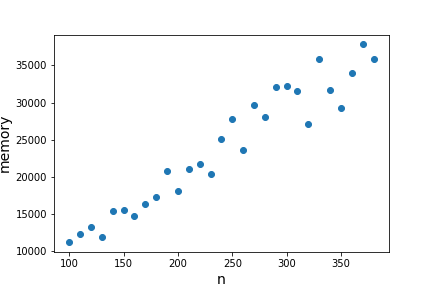
\includegraphics[width=75mm]{fig1.png}}
\subfigure[]{\label{fig:2}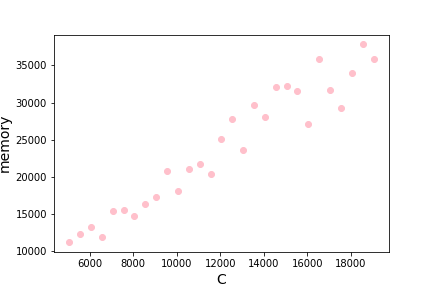
\includegraphics[width=75mm]{fig2.png}}
\caption{Memory used in execution increases along with the increase of $n$ (a) and $C$ (b).}
\end{figure}
\begin{figure}[H]
    \centering
    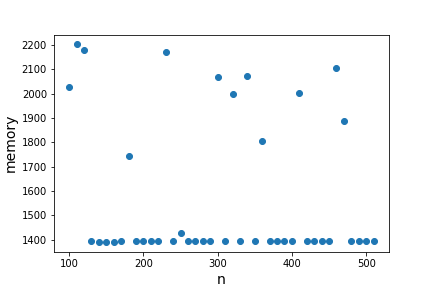
\includegraphics[width=85mm]{fig3.png}
    \caption{Memory in execution stays mostly invariant with fixed $C$ and different values of $n$.}
    \label{fig:3}
\end{figure}

\indent Through experiments, it can be observed that the memory used for the optimized algorithm only depends on $C$ instead of both $n$ and $C$ like the previous approaches. This is also reconcilable with our intuition mentioned above. 

\section{Conclusion}
In this project, we have presented three different approaches to solve knapsack problem, these are: Naive Recursive, Top-down Dynamic Programming \cite{greedy} and Bottom-up Dynamic Programming \cite{budp}.

Naive Recursive approach is a simple brute force algorithm, which considers all subsets of objects, computes all the weights and values and choose the subset which has the greatest value and at the same time has total weight smaller than the knapsack capacity. This approach is easy to implement and to understand in terms of mathematics and idea, but unfortunately since its complexity is large, it does not have remarkable efficiency compared to the other approaches and does not work well with huge inputs.

Top-down Dynamic Programming is a dynamic programming approach, which stores the results of each recursive call in a table and directly return it when needed instead of re-calculate it as Naive Recursive approach. This approach surely improves the complexity and the execution times of the algorithm, therefore achieve better performances.

Bottom-up Dynamic Programming is another dynamic programming approach. Instead of starting from the original problem as Top-down approach, in Bottom-up approach, we start from the smallest sub-problems and solve the bigger problems by those previous ones. This approach also produces a comparable results to Top-down approach.

Among those approaches that we have considered, the two dynamic programming ones definitely have better performances than the Naive Recursive approach, and the optimized ones obtain better space complexity. There are also more approaches to solve the knapsack problem other than those three, some are worse and some are better than ours, including: greedy approach\cite{greedy}, branch and bound approach \cite{bab}, genetic algorithm approach \cite{ga},... 
\printbibliography[title = {References}]


\end{document}
